
\documentclass[11pt]{article}
\usepackage[utf8]{inputenc}
\usepackage{fullpage}
\usepackage{times}
\usepackage{graphicx}
\usepackage{multicol}
\usepackage{amsmath}
\usepackage{tabularx}
\usepackage{setspace}
\usepackage{listings}
\usepackage{mathtools}
\raggedright

\renewcommand{\contentsname}{Innehållsförteckning}
\renewcommand{\figurename}{Figur}
\renewcommand{\tablename}{Tabell}

\lstset{
         basicstyle=\footnotesize\ttfamily, % Standardstil
         %numbers=left,                     % Visa inte radnummer
         numberstyle=\tiny,                 %
         numbersep=5pt,                     %
         tabsize=2,                         % Small tabs
         extendedchars=true,                %
         breaklines=true,                   %
         showspaces=false,                  % Don't show ugly spaces thx
         showtabs=false,                    % Or tabs
         showstringspaces=false             % No spaces here either ffs
         xleftmargin=17pt,
         framexleftmargin=17pt,
         framexrightmargin=5pt,
         framexbottommargin=4pt,
}
\begin{document}

% Frontpage
\begin{titlepage}

\begin{center}


\vspace*{1cm}

% Title
%{ \huge \bfseries Core Wars}\\[0.2cm]
{ \Large \bfseries TSEA43}\\[0.2cm]
{ Projektrapport}\\[0.2cm]


\begin{figure}[h]
    \begin{center}
        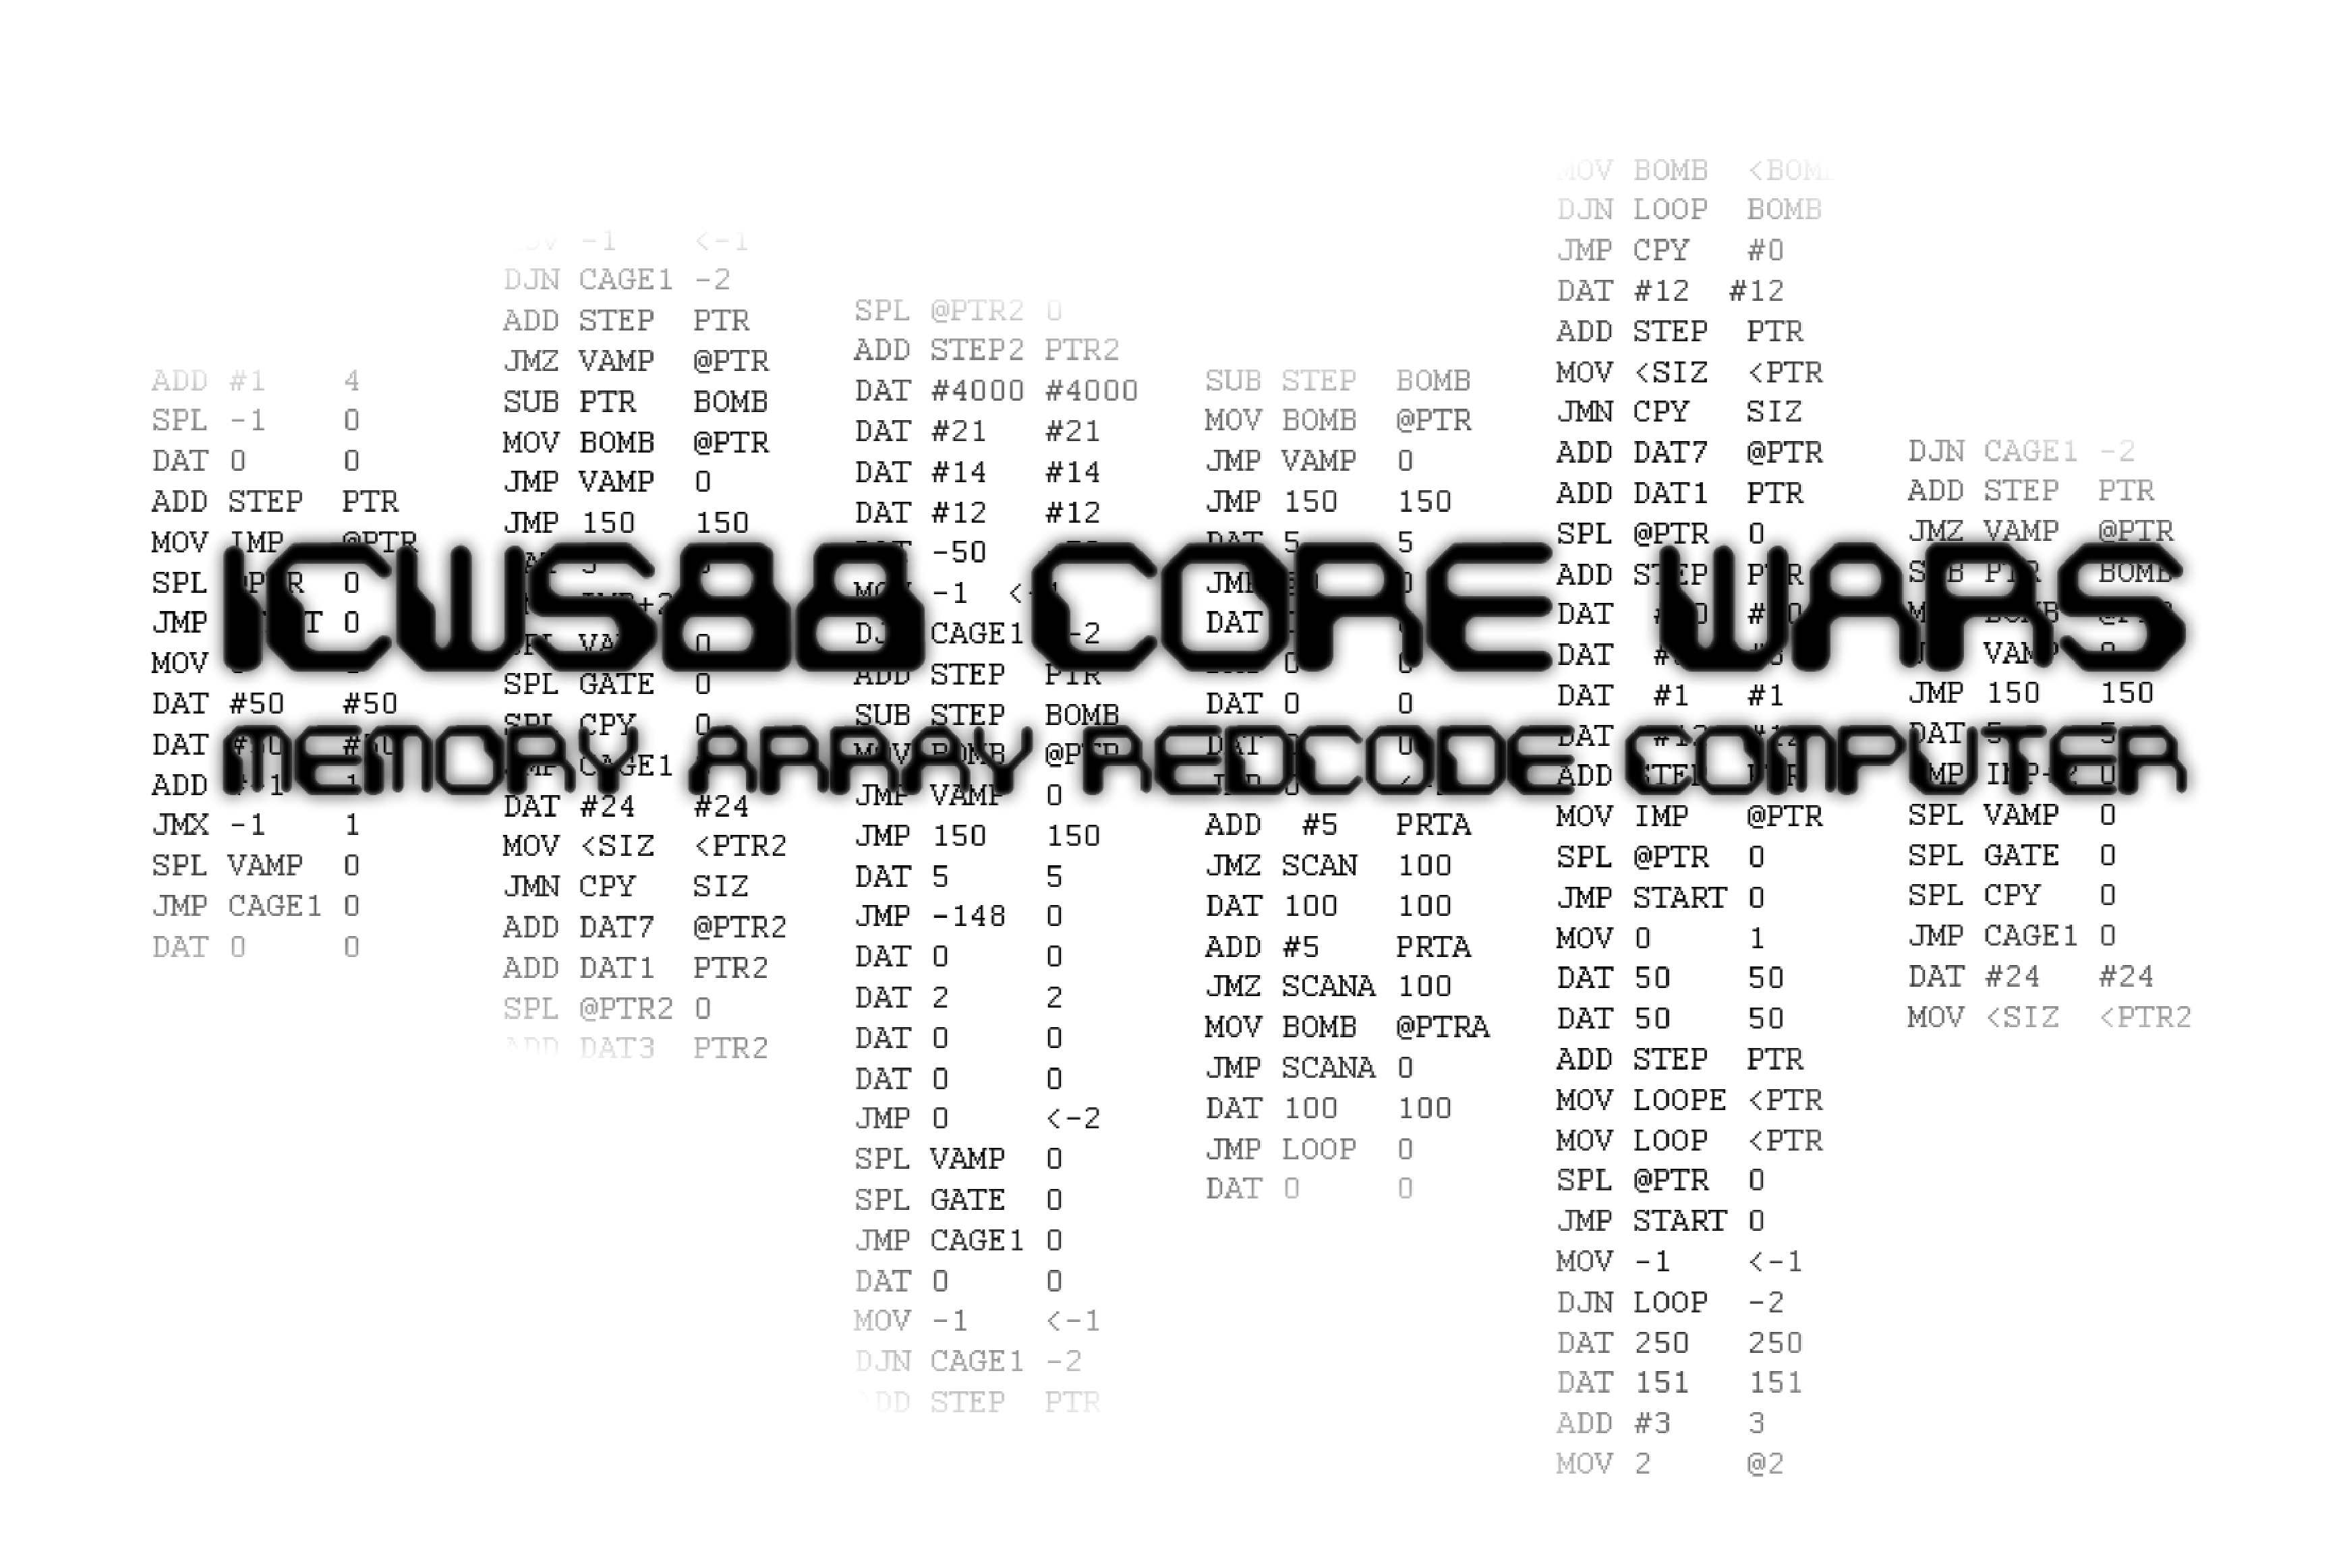
\includegraphics[width=15cm]{Logo01.eps}
        \label{fig:Logo01}
    \end{center}
\end{figure}

\vspace*{2cm}

Jonas Hietala \\
Jesper Tingvall \\
Jizhi Li

\vfill

% Bottom of the page
{\large 15 April, 2012}

\end{center}

\end{titlepage}
\newpage

% empty after frontpage
\newpage
\thispagestyle{empty}
\mbox{}


% 2nd page
\newpage
\section*{Sammanfattning}

I detta projekt har vi byggt en mikrodator som använder Redcode som assembler. Detta för att kunna spela spelet Core Wars. Vi använder en UART för att skriva in koden till datorns minne och vi kan dumpa ut minnesinnehållet och spelets status på en skärm genom VGA-porten. I rapporten går vi igenom lite Redcode, beskrivning av hårdvara till vår mikrodator och hur vi använder RS232 och VGA standarden. Till sist har vi en del exempel Warriors som visar de vanligaste Core Wars strategierna.

\thispagestyle{empty}
\newpage


% 3rd page
\tableofcontents

\thispagestyle{empty}
\newpage


% 4th page. Start page numbering here.
\setcounter{page}{1}
\pagenumbering{arabic}

% Space up paragraphs a bit
\setlength{\parskip}{4mm plus1mm minus3mm}

\section{Inledning}

Vårt mål med projektet i denna TSEA43 kurs var att bygga en dator som kunde köra det eminenta spelet Core Wars. Core Wars är ett ointeraktivt spel där spelarna skriver sina program i Redcode assembler. Målet var att bygga en maskin som använde Redcode som sin assembler och som kunde måla ut spelområdet, d.v.s. minnet, till en VGA skärm och ta emot ny kod via en UART. För mer utförlig information om våra designmål rekommenderas en läsning i vår designskiss \footnote{Se bilaga TODO}.

Vi namnger vår dator till M.A.R.C, Memory Array Redcode Computer då simulatorn heter M.A.R.S, Memory Array Redcode Simulator. Värt att nämna är att Core Wars ej refererat till processor kärnan utan till ett gammalt kärnminne.

Vårt mål är att kunna spela Core Wars enligt 1988 standarden\footnote{http://corewars.nihilists.de/redcode-icws-88.pdf}, skicka in innehåll till M.A.R.C från en kontrolldator och sätta ut två spelares position. Vi vill även kunna dump ut minnesinnehåll och spelstatus till en VGA skärm. Vår uDator skall kunna utföra alla 10 instruktioner och 4 adresseringsmoder Redcode har samt kunna växla mellan, skapa och ta bort processer. Vi rekommenderar en läsning utav 1988 standarden då vi ej kommer att gå igenom instruktionerna eller adresseringsmoderna i denna rapport.

\newpage

% 5th page.
\section{ICWS88 Redcode}

\subsection{Introduktion}
Vi har programmerat en assembler som kan generera en binärfil ifrån två Warriors skrivna i Redcode. Vi randomiserar också deras startläge. Vi kan sedan skicka den assemblerade koden och startpositionerna till MARC genom UART.

\subsection{Exempel Warriors}

\textbf{Replicator} \\
Replicators skapar kopior av sig själva och förökar sig i minnet. De motverkar bombers då bombers inte kan förstöra replicatorn tillräckligt snabbt.

\textbf{Factory Bomber} \\
Factory bomber (eller bomber factory då den bygger bombers) formaterar hela minnet via att masskopiera en massa ’little bombers’ till minnet. Dessa databombar minnet och kommer efter ett tag bomba isär orginalkoden. Denna Warrior är därmed en blandning mellan en bombare och en replicator.

\textbf{Carpet Bomber} \\
Carpet bombers är en blandning mellan en bomber och en scanner. De traverserar minnet och lägger in bombers där minnet har ändrats. Denna Warrior är smartare än en vanlig bomber då den inte kommer att bomba ute i tomma minnet. Den kommer också vara lite snabbare än en traditionell bomber som behöver kopiera ut data.

\textbf{Imp Spawner} \\
Denna Warrior är ej offensiv och har som stategi att skapar en massa imps. Imp spawner fungerar ungefär som Factory Bomber fast har en annan payload.

\textbf{Vampire Bomber Gate Replicator} \\
Denna otympliga Warrior startade som ett skämt då vi ville se vad som hände om man inkluderade så många strategier som möjligt i en Warrior. Dock blev den inte så dålig som vi först trodde. Först så skapar Warriorn en kopia av sig själv, denna kopia kan dock ej kopiera sig själv, något som borde kunna lösas med hjälp av lite hjärnverksamhet och en texteditor. Efter kopiatorn så har Warriorn en ”bomber cage”, dessa två rader databombar minnet bakåt. Efter cagen kommer vampyrkoden. En vampyr JMP bombar minnet i hopp om att fienden skall hoppa in i dess cage. Den kan därmed sno klockcykler ifrån motståndarens kod. Sist finns en gate ifall resten av koden skulle bli överkörd av en Imp.

\newpage

\begin{figure}[h]
    \begin{center}
        
\includegraphics[width=3cm]{Kopimi.eps}
    \end{center}
\end{figure}

\textbf{Kopimi} \\
Denna Warrior scannar minnet efter information, kopierar den och börjar sen exekvera den. Den kan därmed härma en fientlig Warrior om den skulle hitta den. Fungerar skapligt trots att den utvecklades mest för att se vad som hände om man skulle tolka Det Missionerande Kopimistsamfundet missionsbudskap\footnote{http://kopimistsamfundet.se}; ”Kopiera och sprid” i form av Redcode. Denna Warrior använder replicator strategin.

\textbf{Inseminator} \\
Ännu en Warrior som skapades på skoj men som visade sig vara rätt så effektiv. Den letar upp motståndarens kod och injicerar en massa processer i den i hopp om att motståndaren ej ska förstöra sig egen kod. Detta brukar dock förstöra funktionaliteten i motståndarens kod då den förutsätter oftast att koden exekveras sekventiellt.

\textbf{Core Cleaner} \\
En core cleaner är ett program som databombar hela minnet. Ofta går man igenom minnet två gånger, den första fyller man minnet med split instruktioner för att slöa ner motståndaren och sedan med DAT-instruktioner för att göra slut på honom.

\textbf{Dwarf Scout} \\
En dwarf scout är en enkel bomber som skyddar sig mot andra bombers genom att se om någon ändrar i minnet i dess närhet. Om så är fallet så kommer den att hoppa till en ny plats i minnet och ta med sig sina processer.

\newpage

\section{Teori}

\subsection{VGA}

\begin{figure}[h]
    \begin{center}
        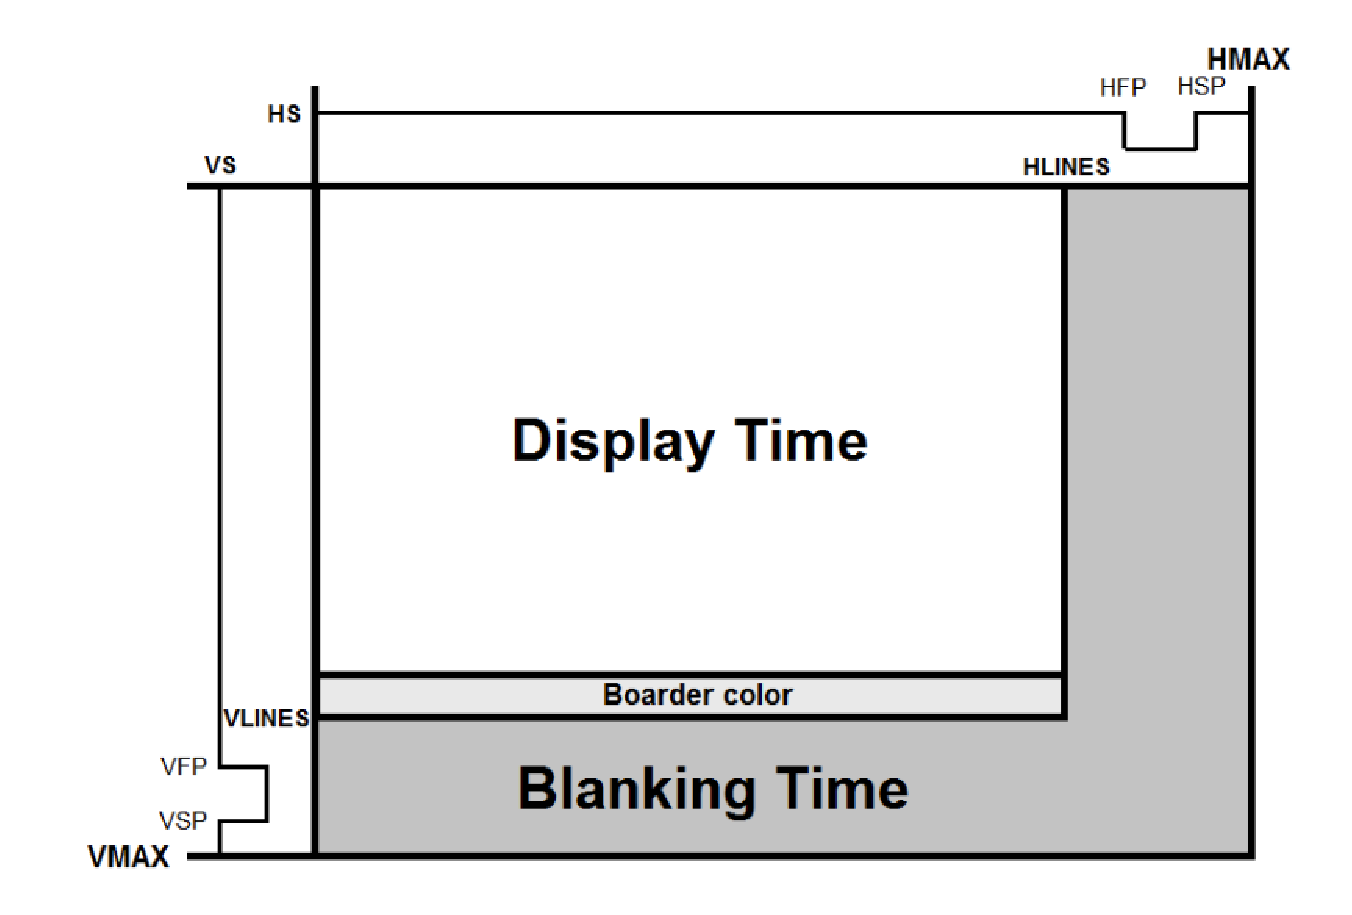
\includegraphics[width=11cm]{display_timing.eps}
        \caption{Display timing}
        \label{fig:display_timing}
    \end{center}
\end{figure}

När VGA skickar pixeldata till VGA porten kommer skärmen inte ta emot och visa pixel data under hela tiden. Dessutom finns det en speciell timing till olika upplösningar med olika frekvenser. Upplösning 640x480 med frekvens 60Hz har vi följande timing enligt Digilent®.

\begin{itemize}
    \item HMAX: 800
    \item VMAX: 525
    \item HLINES: 640
    \item VLINES: 480
    \item HFP: 648
    \item HSP: 744
    \item VFP: 482
    \item VSP: 484
    \item Clk: 25MHz
\end{itemize}

Vi har blanking time för att en skärm använder en stråle för att visa varje pixel och strålen flyttar sig från vänster till höger och sedan ner på nästa rad och upprepar denna process. Under blanking time kommer strålen flytta sig från höger till vänster och under denna tid ska skärmen inte visar någon pixel. Mellan front porch och back porch går sync signal ner och upp igen på grund av att det är sync signal som uppdaterar och bestämmer frekvens till skärmen.

På display ytan, kommer varje pixel uppdateras enligt den 8 bitars färg som skärmen har fått genom VGA porten och på blank ytan ska vga porten får ingen färg data alls, annars kommer skärmen visa denna färg när de flyttar sig tillbaka över skärmen.

\subsection{RS232}

Vårt FPGA kort har en USB till RS232 port. Vi använde denna för att föra över den assemblerade spelarkoden till kortet. En överförning inleds av en startbit, därefter följer 8 databitar och en stoppbit. Hastigheten mäts i baud, tecken (på 8 bitar) per sekund. I vårt fall var ledningen hög när ingen överförning var igång (1). Överförningen inleds med att ledningen jordas (2), därefter följer 8 databitar i vald hastighet (3). I slutet av överförningen kommer en stoppbit som är hög (4). Se figur \ref{fig:rs232}.

\begin{figure}[h]
    \begin{center}
        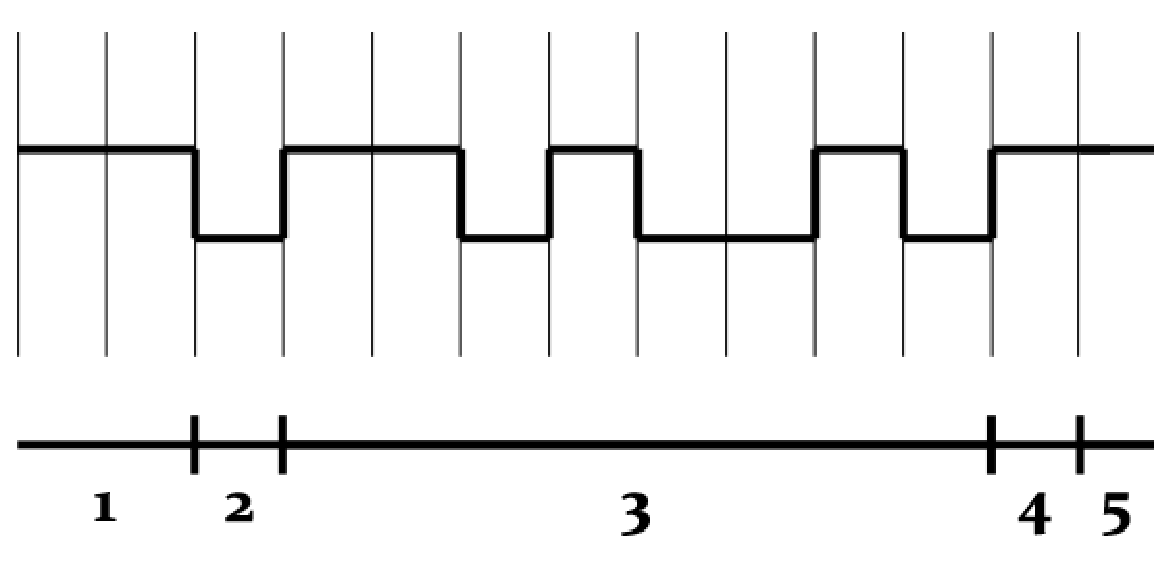
\includegraphics[width=10cm]{rs232.eps}
        \caption{En RS232 överförning. Man har ingen gemensam klocka för sändare och mottagare utan överför endast data, sändaren och mottagaren känner dock till vilken baud rate man överför med. I vårt fall använder vi 115 200 baud.}
        \label{fig:rs232}
    \end{center}
\end{figure}

\newpage


\section{Beskrivning av hårdvara (M.A.R.C)}

\subsection{Mikrodatorn}

Datorn är en mikroprogrammerad dator med 39 styrsignaler + 8 signaler för hoppaddresser. Mikrominnet är 256 rader långt och mer än 200 rader är använt. Dess huduvuppgifter är att nollställa minnet vid en reset, slussa in program i minnet vid inladdning via fbart och hämtning och exekverande av instruktioner.

\begin{figure}[h]
    \begin{center}
        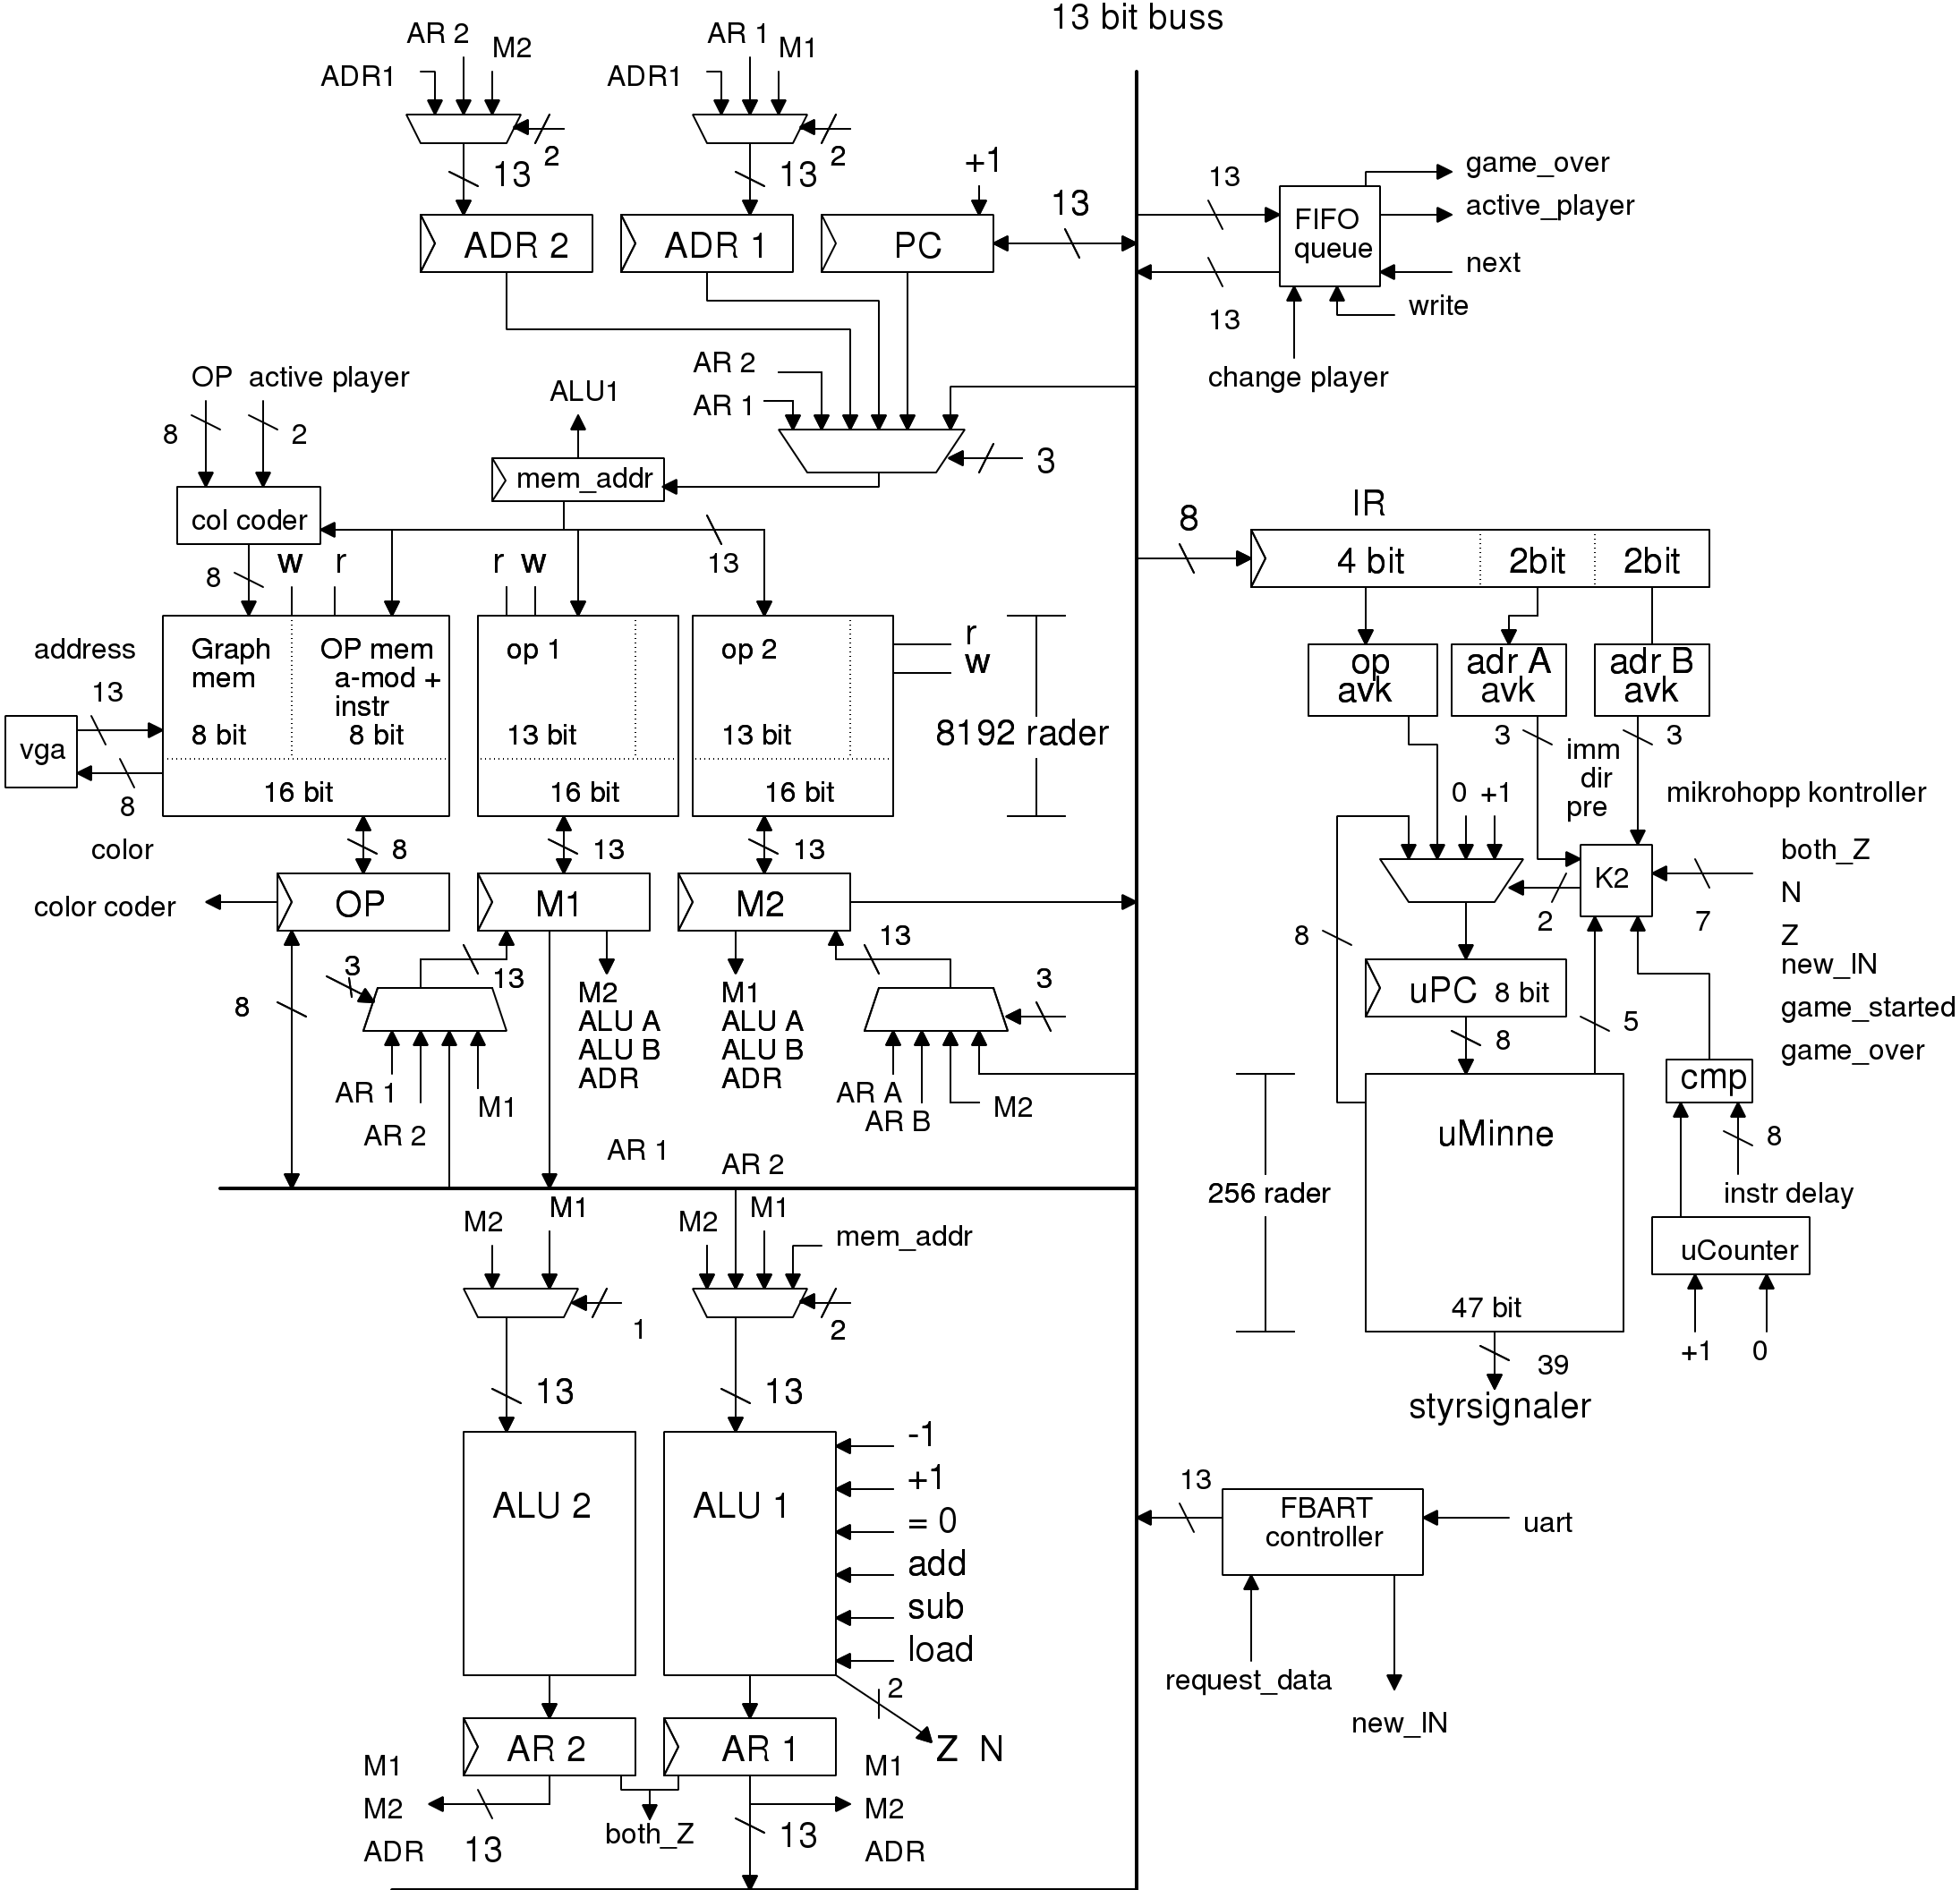
\includegraphics[width=16cm]{huvudblockschema.eps}
        \caption{Huvudblockschema}
        \label{fig:huvud}
    \end{center}
\end{figure}

% Formating
\newpage

Blockschemat beskriver vilka register (alla osynliga för programmeraren) som finns och hur de är kopplade med omgivningen. Det finns två ALU:s för att korta ner på antalet klockcykler det krävs för att göra parallella operationer på A och B operanderna. På samma sätt har de flesta registren multiplexade ingångar för att spara tid och för att öka förmågan för parallellism.

Mikrominnet har en mängd olika hopp som den kan göra, den kan bland annat hoppa på både A och B's olika adresseringsmoder eller ALU:ns olika flaggor. För att sakta ner exekveringen fördröjs exekveringen av varje instruktion genom att jämföra en räknare med en fördröjningssignal "instr delay". Detta för man ska kunna följa spelet gång på skärmen.

Vid exekvering av en instruktion laddas instruktionen först in till IR, sedan beräknas adresseringsmoderna för A och B och därefter utförs instruktionen. Adressmodsberäkningen är besvärlig då både A och B operanderna kan vara en av de fyra olika moderna. Detta kompliceras ytterligare då vissa instruktioner gör olika saker beroende på vilka adresseringsmoder som används. Efter beräkningen lagras operanderna i M1 och M2, om immediate, och annars i adressregistren ADR1 och ADR2. Schemat visar även var vga, FIFO och fbart controller ansluts.

\newpage
\subsection{VGA}

VGA är uppdelad i två delar: vga\_controller och pixelsender. Vga\_controller tar hand om timing av signaler till VGA-port och pixelsender använder samma timing som vga\_controller samt hämta färg data urifrån huvudminne. Se figur \ref{fig:vga2} för detaljer.

I vga\_controller finns det två räknare: h\_counter som räknar antalet horisontella pixlar och v\_counter som räknar antalet vertikala pixlar. Varje gång när h\_counter räknar upp till HMAX, dvs. maximalt antal pixlar på en rad, så kommer h\_counter nollställas och skicka en +1 insignal till v\_counter; v\_counter kommer att nollställas när den uppnå VMAX. (antalet pixel för varje kolumn)

HFP(slutpunkt till horisontal front porch), HSP(slutpunkt till horisontal synkpuls), VFP(slutpunkt till vertikal front porch), VSP(slutpunkt till vertikal synkpuls) kommer vi att använda i vga\_controller. HFP kommer att aktiveras när h\_counter > HFP och skicka jordsignal till H-sync och HSP kommer att aktiveras när h\_counter > HSP eller h\_counter < HFP och skicka högsignal till H-sync. VFP och VSP kommer att skicka sync signal till V-sync med på samma sätt.

\begin{figure}[h]
    \begin{center}
        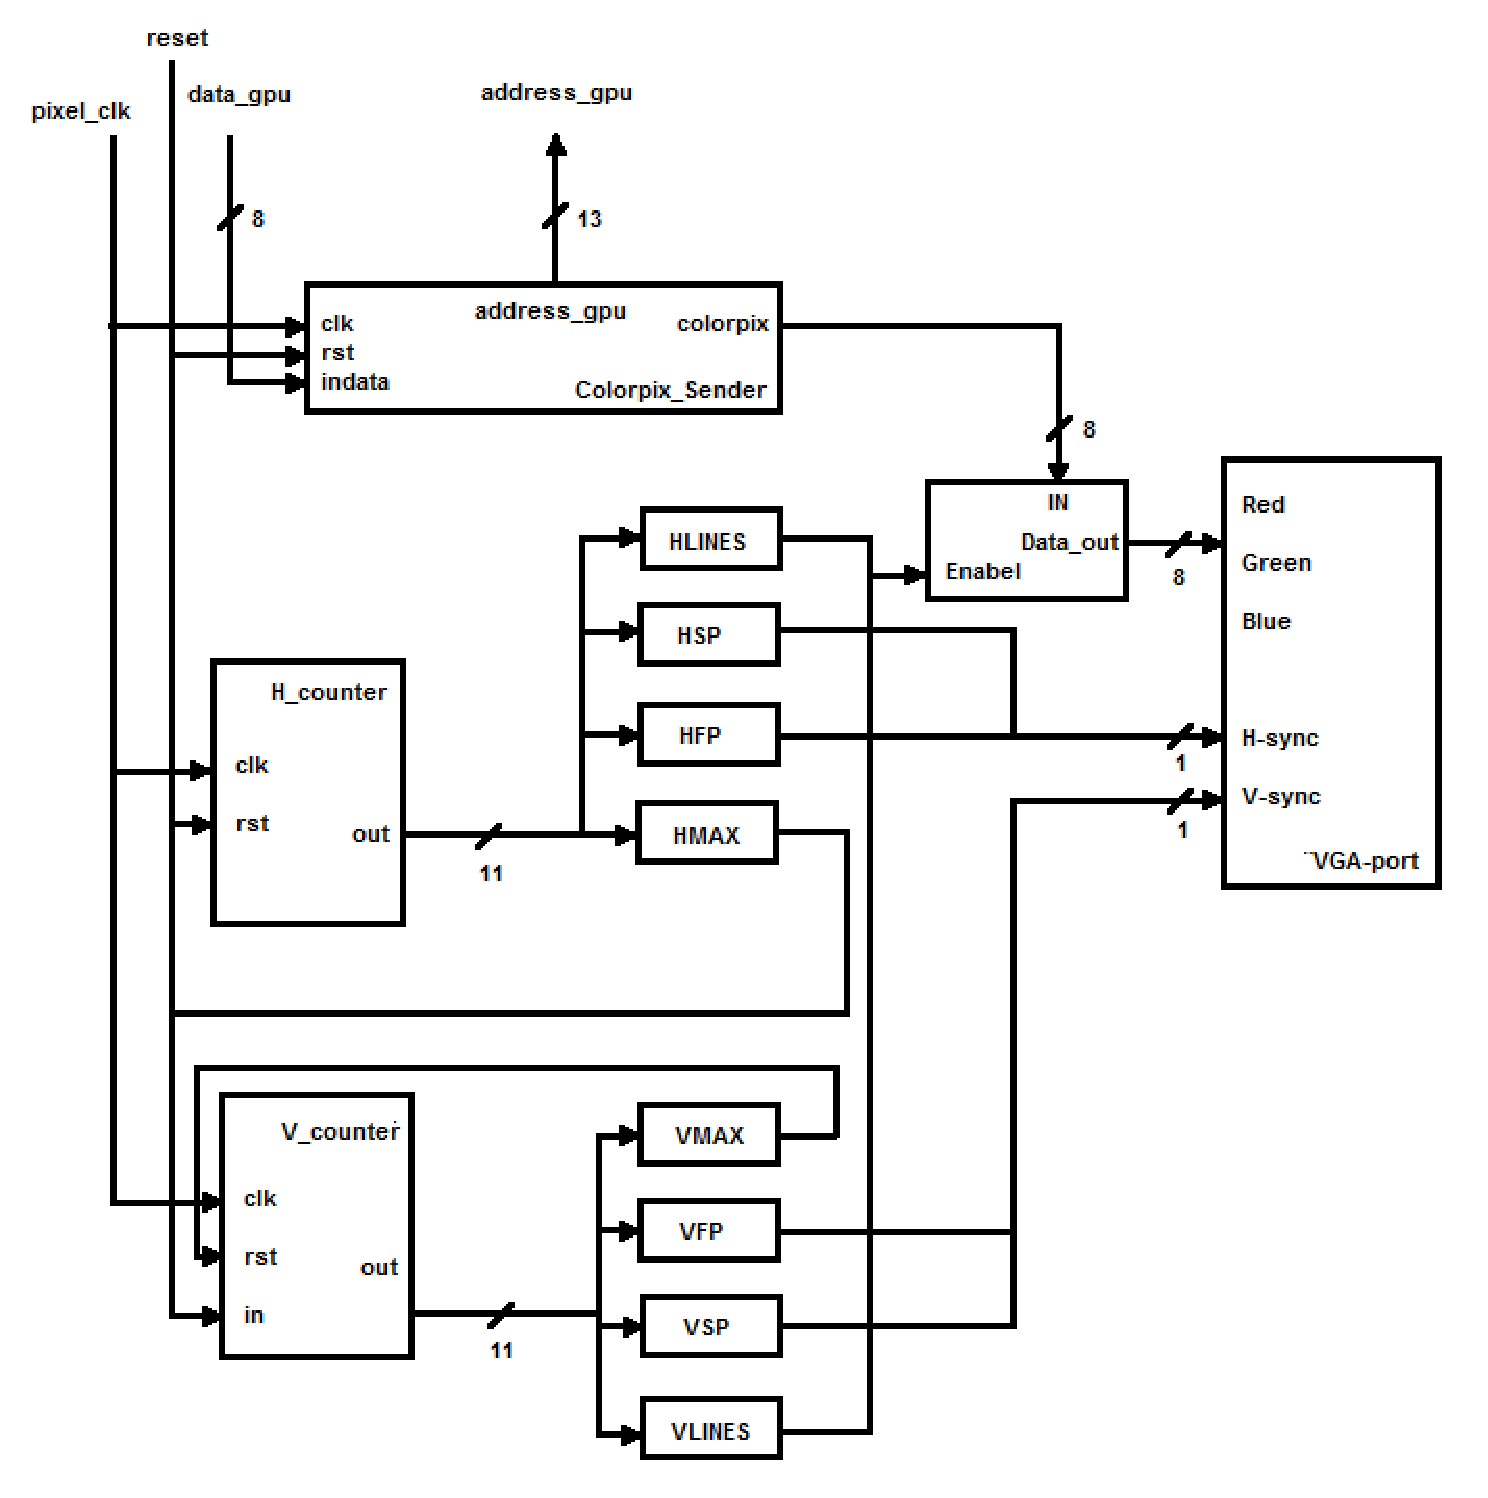
\includegraphics[width=11cm]{vga2.eps}
        \caption{VGA blockschema}
        \label{fig:vga2}
    \end{center}
\end{figure}

% Formating
\vspace{4cm}

VGA-port kommer endast ta emot färg data när h\_counter < HLINES(640 enligt upplösning vi valde) och v\_counter < VLINES(480 enligt upplösning vi valde) med hjälp av en enable signal från HLINE och VLINE.
Pixelsender använder samma timing och klocka som vga\_controller och skickar en 13 bitars adress till vårt färgminne, hämtar 8 bitars data på detta adress och då skickar denna data till vga-porten endast när räknare in vga\_controller ligger inom display-ytan.

PixelSender tar hand om address hämtning och färg kod sändning. För att alla data i minnet ska se bra ut på skärmen bestämde vi att visa varje instruktion ska vara 5 pixlar bred och 7 pixlar hög. I så fall kommer vi att visa 128 data per rad och vi behöver 7*64 = 448 rader för att visa 213 = 8192 adresser. PixelSender skickar data till skärmen var 5:e klockpuls och upprepar detta för varje 128 data 7 gånger, i så fall kan vi ha varje instruktion med 5*7 pixel storlek. På ”border area” visar vi vilken spelare vinner CoreWar.

\newpage
\subsection{Minnen}

Vi valde att använda en core size (storlek på spelplan) på 8192 rader, detta brukar vara standard i duell spel men ibland avrundar man till 8000 rader. Om man kör fler än 2 spelare brukar minnet vara betyderlig större, vi ska dock endast ha 2 spelare stöd. Vi behöver enligt (1) 13 bitar för att kunna adressera hela detta område. Då minnet i FPGAN är indelade i block mindre än detta fick vi dela upp minnet på flera block.

Varje rad Redcode delades upp i 4 delar; instruktion och adresseringsmoder på 8 bitar, operand A på 13 bitar, operand B på 13 bitar och 8 bitar RGB färgning. Det som bäst stämde överens med vår uppdelning var att använda minnesblock utav storleken 1024 x 16 bitar (de 3 sista bitarna används ej dock i operandminnena), se figur \ref{fig:memory_cell}.

\begin{figure}[h]
    \begin{center}
        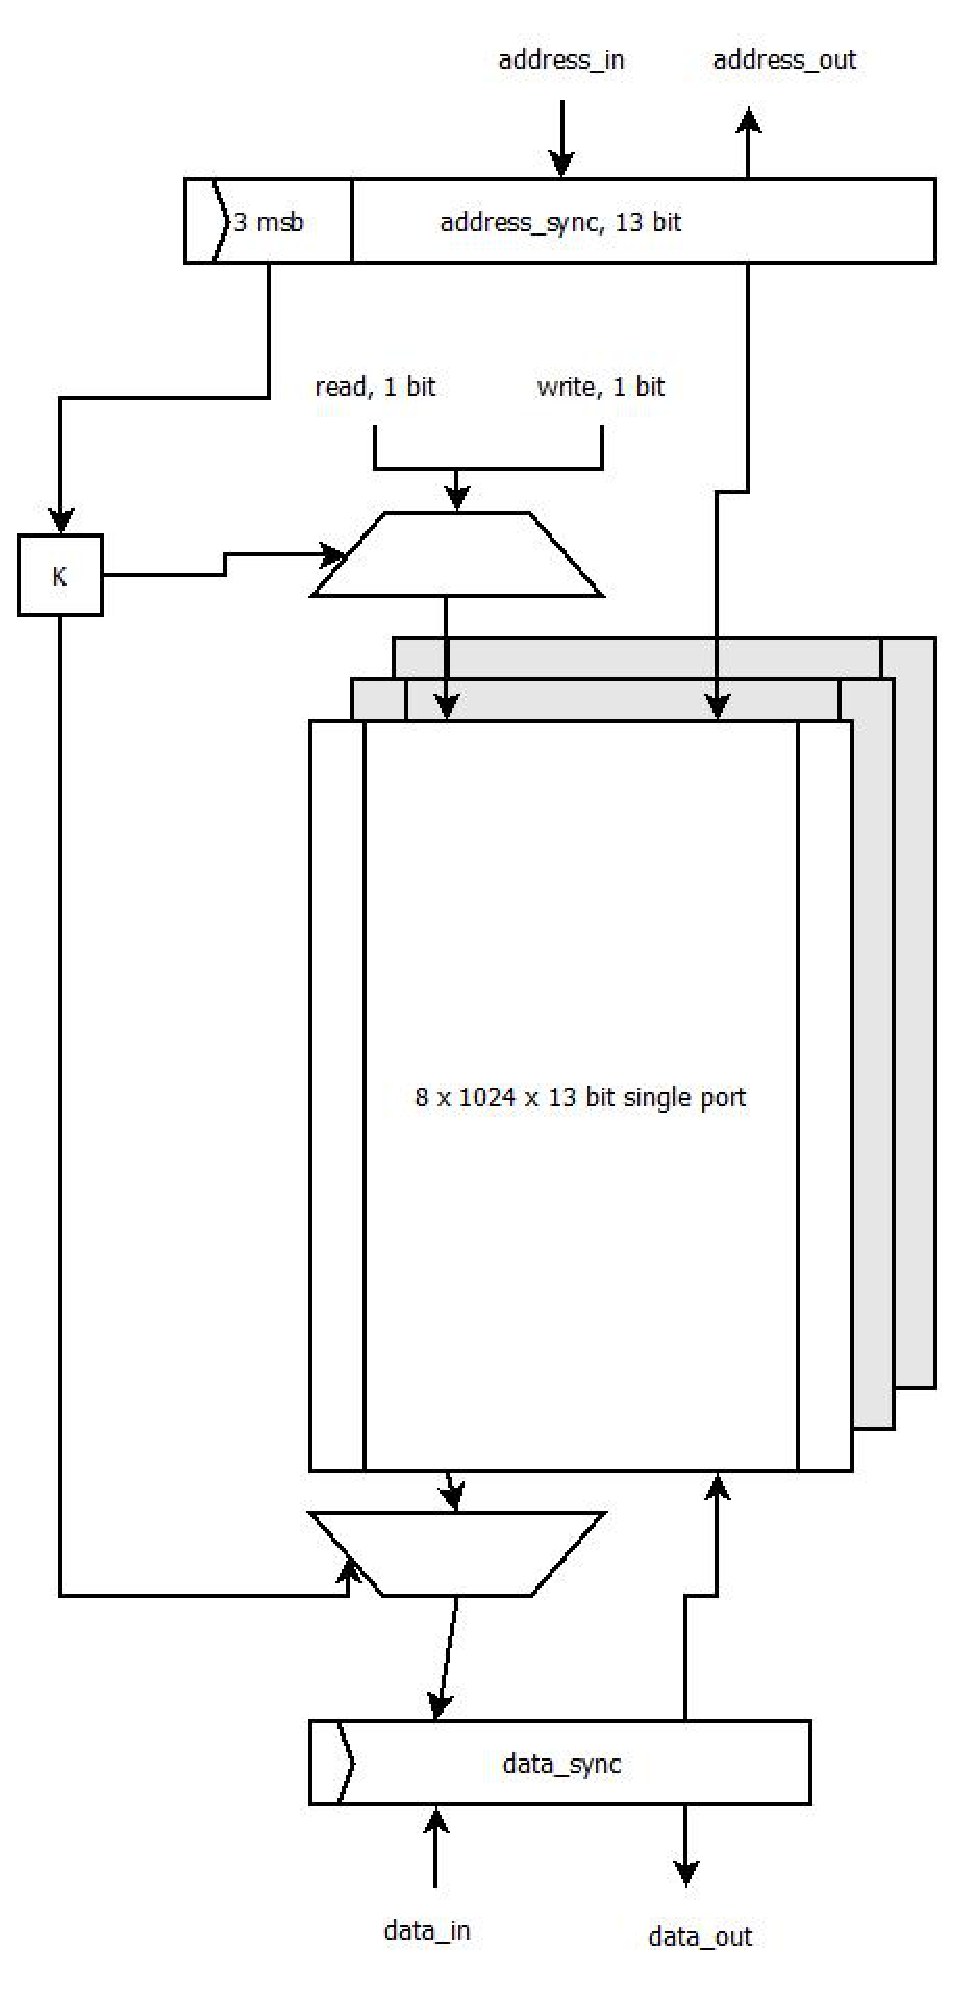
\includegraphics[width=6cm]{memory_cell.eps}
        \caption{Operandminnen}
        \label{fig:memory_cell}
    \end{center}
\end{figure}

De tre mest signifikanta bitarna styr multiplexern och ser till att rätt minne skriver och läses ifrån. Våra minnen var lite bättre än vad vi först förväntade oss, därför har vi en adress\_sync och data\_sync register, vi skulle kunna ta bort dessa och därmed snabba upp datorns minnesaccess.

Då vi har olika färg beroende på vilken instruktion vi har i instruktionsminnet var det naturligt att slå samman instruktionsminnet och färgminnet då båda var på 8 bitar. Den resulterande maskinen ses i figur \ref{fig:memory_cell_dual}. Skillnaden mellan den och operandminnena är att den använder ett dualportminne med den andra adressingången kopplad till GPUn. Färgen skrivs automatiskt till minnet när man skriver in en instruktion i minnet.

\begin{figure}[h]
    \begin{center}
        \includegraphics[width=10cm]{memory_cell_dual.eps}
        \caption{Instruktions och färgminne}
        \label{fig:memory_cell_dual}
    \end{center}
\end{figure}

\newpage
\subsection{UART}

Vår dator använder en 13 bitars buss, det skulle därmed vara trevligt om indatat ifrån vår värddator skulle vara 13 bitar detta med. Då vi använder Anders Nilssons FBART vilken arbetar i 8 bitar skulle det vara trevligt att slå samman två sändningar till en. Det gör vi med modulen i figur \ref{fig:uart}. Modulen väntar på en databegäran, tar emot två 8 bitars överförningar, slår samman dem till 13 bitar (den kastar iväg 3 bitar) och signalerar att data finns.

\begin{figure}[h]
    \begin{center}
        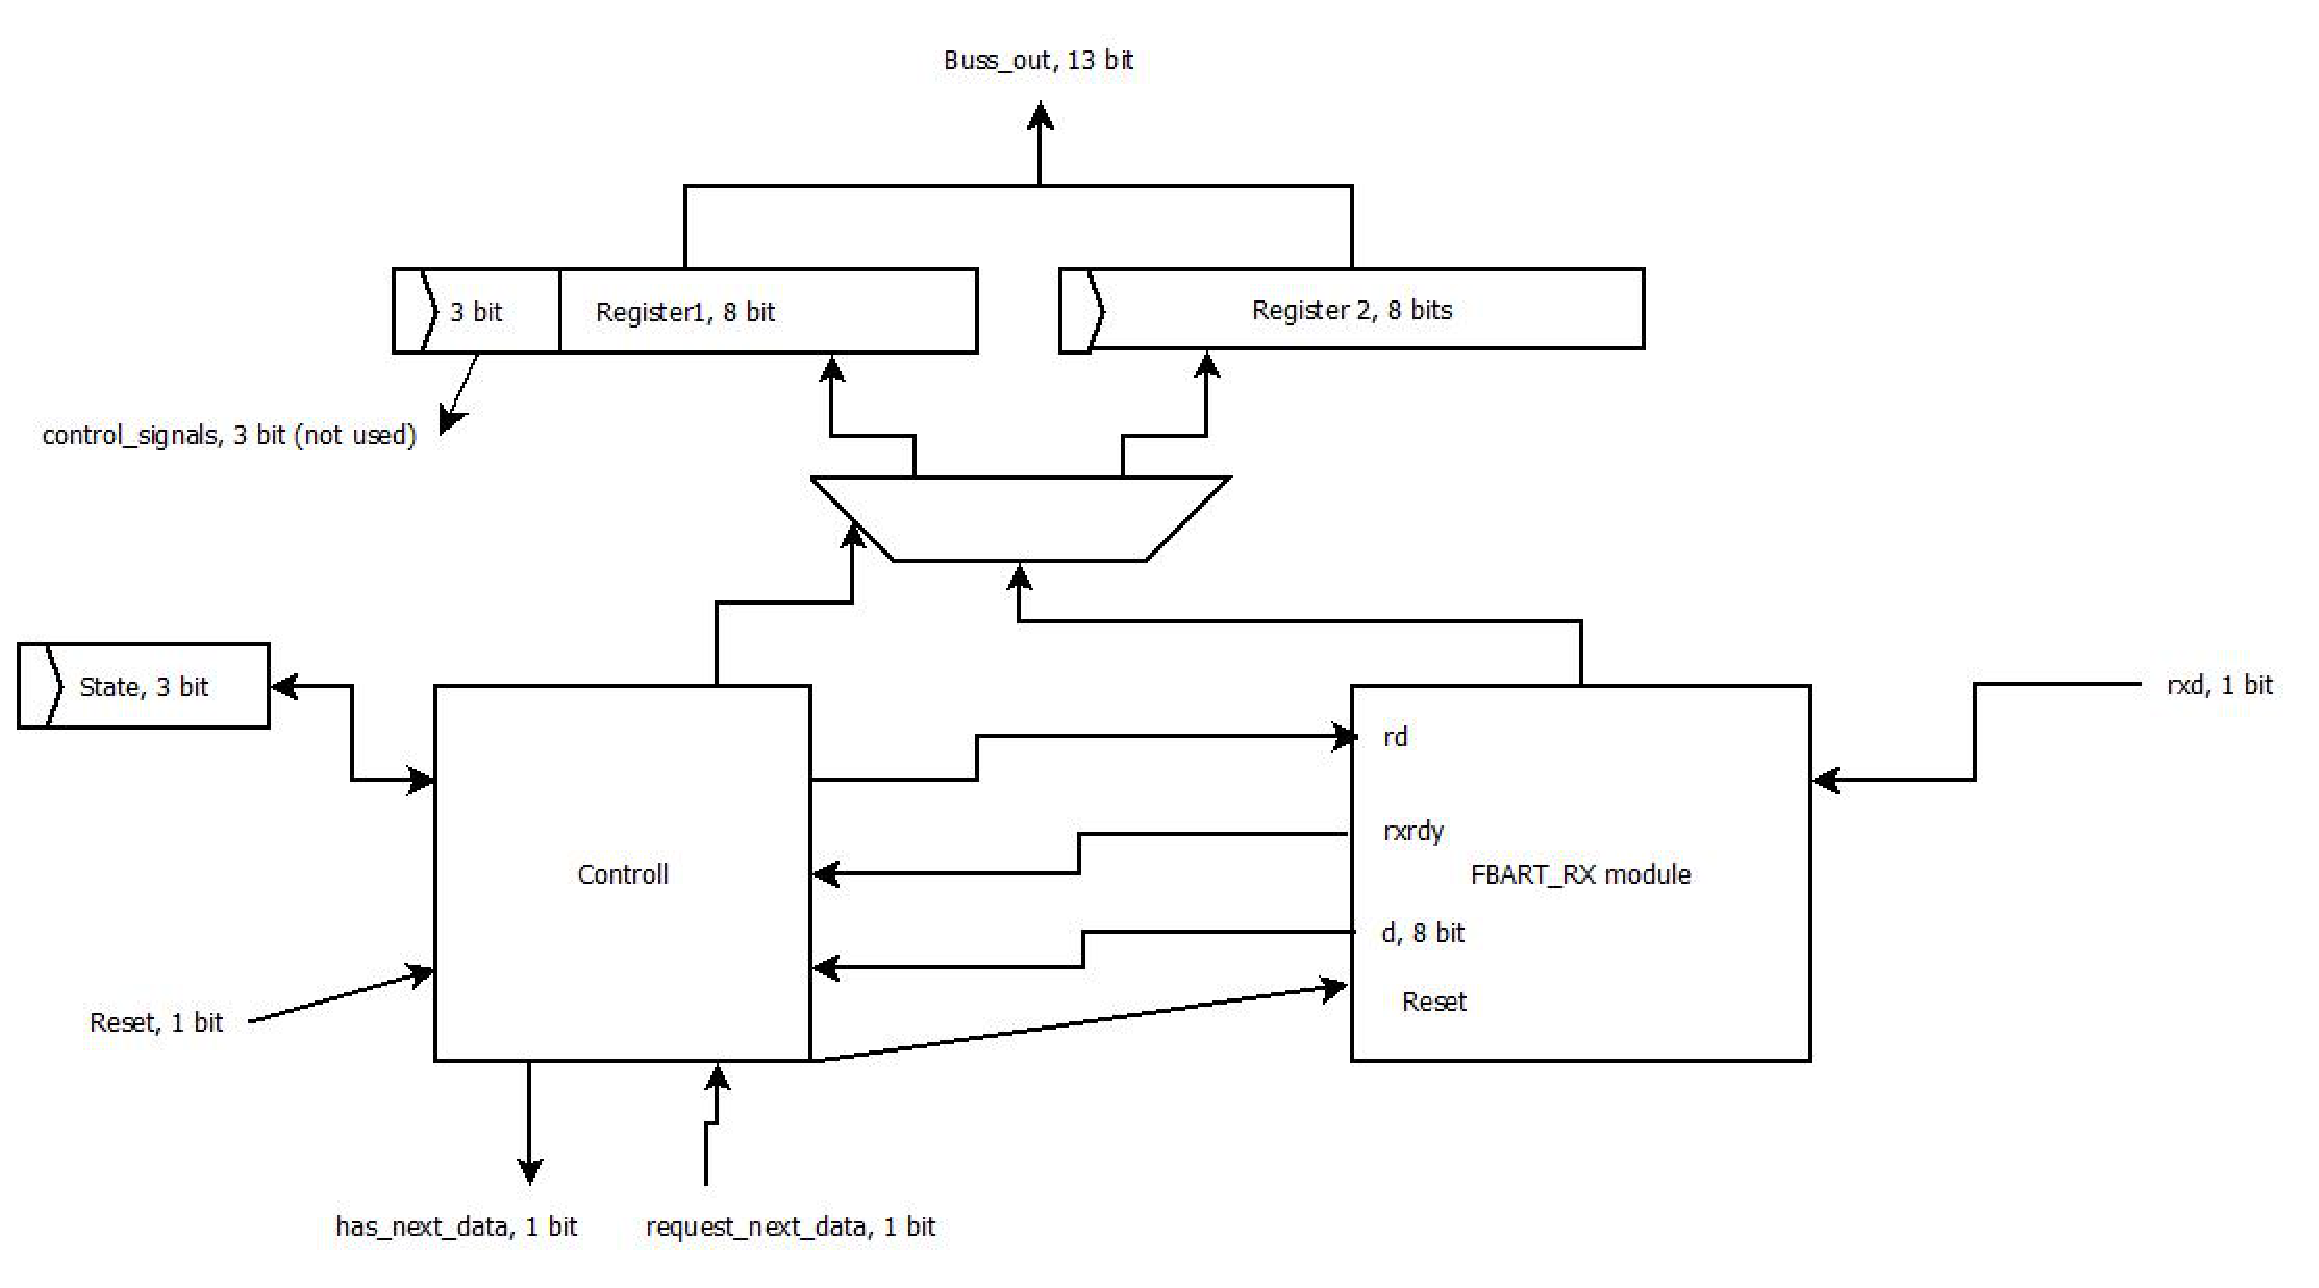
\includegraphics[width=13cm]{uart.eps}
        \caption{UART kontrollerare. Vi fick även ändra i FBARTen då den gick på en 25 MHz klocka och vårt bygge kör på en 100 MHz klocka. Vi behövde endast öka antalet bitar i en räknare och ändra på en konstant.}
        \label{fig:uart}
    \end{center}
\end{figure}

\newpage
\subsection{FIFO}

Då en spelare kan ha flera olika processer igång behöver vi ett sätt att lagra alla programräknare. Vi har implementerat två stycken ”first in first out” köer i vår hårdvara, se figur \ref{fig:fifo}.

\begin{figure}[h]
    \begin{center}
        \includegraphics[width=14cm]{fifo.eps}
        \caption{Player FIFOs.}
        \label{fig:fifo}
    \end{center}
\end{figure}

Headregistret pekar på den översta programräknaren och tailregistret pekar på en sista. När man begär nästa programräknare ökas den nuvarande spelarens head och den översta PCn skrivs till current\_pc\_out. När man skriver in en PC kollas först att den nuvarande spelars kö ej är full, om den ej är full skrivs PC in och tailregistret ökas. Om kön är full görs ingenting. Om någon spelares kö är tom, dvs. headregistret är lika med tailsregistret så signaleras game\_over. Man kan även byta aktiv spelare.


\newpage

\section{Slutsatser}

Arbetet med projektet gick bra, VHDL var lite motsträvigt men vi lyckades implementera hela CoreWars 1988 standarden och få våra Redcode Warriors att fungera. Core Wars var väldigt kul, både att implementera och att skapa Warriors till.

Implementationen skulle kunna förbättras. Mikrokodningen är inte alls optimerad då det kändes lite onödigt då vi hade en 27 bitars delayräknare efter varje exekverad instruktion. Minnesaccessen skulle kunna förbättras och VHDL koden är onödigt komplex på flera ställen.

Vid fortsatt arbete kan mikrokoden göras snabbare genom mikrokodsoptimering. Till exempel skulle man kunna ha parallell adressavkodning då vi har dubbla ALUs. En nyare standard skulle kunna implementeras då den ger möjligheter till nya variationer av Warriors. Det finns regler om timeouts som vi inte tar hänsyn till. Om kommunikationen till datorn skulle kunna utökas skulle MARC kunna användas som en King of the Hill server för att ställa Warriors mot varandra och ranka dem. Man skulle kunna utöka stödet till mer än två spelare och köra en Free For All. En utökad core size och stöd för fler samtidiga processer skulle kunna läggas till.

\newpage

% Appendix here
\appendix
\section{Warriors}

% Warriors of the world!

% stones

\subsection{Little bomber}
\lstinputlisting{../scripts/j3x-little_bomber.red}

\subsection{Factory bomber}
\lstinputlisting{../scripts/j3x-factory-bomber.red}

\subsection{Carpet bomber}
\lstinputlisting{../scripts/jonas-carpet-bomber.red}

\newpage
\subsection{Core Cleaner}
\lstinputlisting{../scripts/jonas-cleaner.red}

\subsection{Dwarf scout}
\lstinputlisting{../scripts/jonas-dwarfscout.red}

\subsection{Stone of ages}
\lstinputlisting{../scripts/jonas-stone-of-ages.red}

% paper

\newpage
\subsection{Jumper}
\lstinputlisting{../scripts/j3x-jumper.red}

\subsection{Jumper gate}
\lstinputlisting{../scripts/j3x-jumper-gate.red}

\subsection{Inseminator}
\lstinputlisting{../scripts/j3x-inseminator.red}

\subsection{Kopimi}
\lstinputlisting{../scripts/j3x-kopimi.red}

\subsection{Replicator}
\lstinputlisting{../scripts/jonas-replicator.red}

% scissors

\subsection{Scanner}
\lstinputlisting{../scripts/j3x-scanner1.red}

\subsection{Vampire}
\lstinputlisting{../scripts/j3x-vampire.red}

\subsection{Suck on this}
\lstinputlisting{../scripts/jonas-suck-on-this.red}

% mixes +imps

\newpage
\subsection{Imp spawner}
\lstinputlisting{../scripts/j3x-imp-spawner.red}

\subsection{Imp worm}
\lstinputlisting{../scripts/jonas-impworm.red}

\subsection{Vampire bomber}
\lstinputlisting{../scripts/j3x-vampire-bomber.red}

\newpage
\subsection{Vampire bomber gate}
\lstinputlisting{../scripts/j3x-vampire-bomber-gate.red}

\subsection{Vampire bomber gate replicator}
\lstinputlisting{../scripts/j3x-vampire-bomber-gate-replicator.red}

\subsection{The big maker}
\lstinputlisting{../scripts/jonas-the-big-maker.red}


\newpage
\section{VHDL}

% main computer
\subsection{MARC.vhd}
\lstinputlisting[language=VHDL]{../src/MARC/MARC.vhd}

\newpage
\subsection{microcontroller.vhd}
\lstinputlisting[language=VHDL]{../src/MARC/microcontroller.vhd}

\newpage
\subsection{ALU.vhd}
\lstinputlisting[language=VHDL]{../src/MARC/ALU.vhd}

% Memory
\newpage
\subsection{MemoryCell.vhd}
\lstinputlisting[language=VHDL]{../src/MARC/MemoryCell.vhd}

\newpage
\subsection{MemoryCellDualPort.vhd}
\lstinputlisting[language=VHDL]{../src/MARC/MemoryCellDualPort.vhd}

% aux stuff

% fifo
\newpage
\subsection{PlayerFIFO.vhd}
\lstinputlisting[language=VHDL]{../src/MARC/PlayerFIFO.vhd}

% fbart
\newpage
\subsection{FBARTController.vhd}
\lstinputlisting[language=VHDL]{../src/MARC/FBARTController.vhd}

% VGA stuff here
\newpage
\subsection{vga.vhd}
\lstinputlisting[language=VHDL]{../src/MARC/vga.vhd}

\newpage
\subsection{colorpixSender.vhd}
\lstinputlisting[language=VHDL]{../src/MARC/colorpixSender.vhd}

\newpage
\subsection{vgaController.vhd}
\lstinputlisting[language=VHDL]{../src/MARC/vgaController.vhd}

% led
\newpage
\subsection{MARCled.vhd}
\lstinputlisting[language=VHDL]{../src/MARC/MARCled.vhd}


% Scripts
\newpage
\section{Script}

\subsection{Assembler}
\lstinputlisting[language=Perl]{../scripts/assembler}

\newpage
\subsection{Mikrokod}
\lstinputlisting{../scripts/microcode}

\newpage
\subsection{Mikrokodningshjälp}
\lstinputlisting[language=Perl]{../scripts/control_codes}

\end{document}


% Used software
\newpage
\section{Använda mjukvaror}

\begin{itemize}
    \item Xilinx ISE Design Suite 13.4 Webpack
    \item ModelSim Student Edition 10.1b
    \item Digilent ADEPT
    \item Fbart\footnote{Tillhandhållen VHDL kod för att kommunicera med UART.}
\end{itemize}

